\documentclass[a4paper,12pt]{article}
\usepackage[utf8]{inputenc}
\usepackage[T1]{fontenc}
\usepackage[portuguese]{babel}
\usepackage{geometry}
\geometry{margin=2.5cm}
\usepackage{graphicx}
\usepackage{hyperref}
\usepackage{titlesec}
\usepackage{enumitem}

% Pacote para definir a fonte como Times (semelhante ao Times New Roman)
\usepackage{mathptmx}

\title{\textbf{Introdução e Fundamentação Teórica}}
\author{Gabriel Brum}
\date{\today}

\begin{document}

\maketitle

\section{Introdução}
O campo da Aprendizagem de Máquina (Machine Learning) revolucionou diversas áreas; no entanto, o processo manual de desenhar e otimizar modelos exige perícia especializada. Para enfrentar estes desafios, surgiu o AutoML, em que o aprendizado é feito automaticamente sem a escolha prévia de um especialista, sendo a \textit{Neural Architecture Search} (NAS) um subcampo focado na automatização do design das arquiteturas das redes neurais.

\section{Fundamentação Teórica}

\subsection{\textit{Search Space} (SSp)}
O Espaço de Busca (SSp) define o conjunto de todos os hiperparâmetros e arquiteturas possíveis que podem ser formados, incluindo tipos de camadas, conexões e funções de ativação. Um SSp amplo garante a presença de modelos otimizados, mas pode tornar a exploração infinita. As principais categorias de SSp são:
\begin{itemize}[noitemsep]
    \item \textbf{\textit{Layer-based}:} Cada camada só se conecta com a sua respectiva próxima camada. Assim, o otimizador é obrigado a procurar arquiteturas em série (Figura 1). Tem um exemplo (\url{https://arxiv.org/abs/1812.03443}) que fixou para 22 camadas e cada tipo de camada pode ser escolhido entre nove opções diferentes. Desta forma, limitando as opções, o tempo de busca é reduzido.
    \begin{figure}[h]
        \centering
        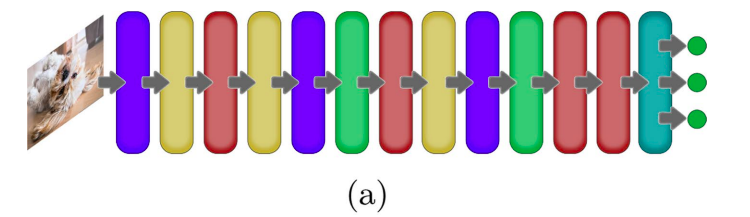
\includegraphics[width=0.5\textwidth]{images/ssp_layer_based.png}
        \caption{Exemplo de arquitetura Layer-based.}
    \end{figure}

    \item \textbf{\textit{Hierarchical-based}:} Além das conexões em série, o modelo pode ter ramificações paralelas e \textit{skip connections} (Figura 2). Como o espaço amostral é aumentado, necessita-se de técnicas para reduzir o tempo de processamento (\url{https://arxiv.org/abs/1807.11626} e \url{https://arxiv.org/abs/1912.00195}).
    \begin{figure}[h]
        \centering
        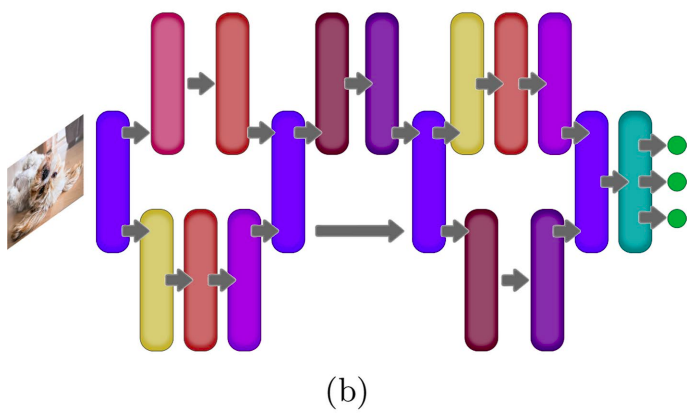
\includegraphics[width=0.5\textwidth]{images/ssp_hierarchical_based.png}
        \caption{Exemplo de arquitetura Hierarchical-based.}
    \end{figure}    

    \item \textbf{\textit{Cell-based}:} A unidade de seleção é uma célula que será conectada em série para criar modelos com diferentes tamanhos (Figura 3). Entretanto, as camadas em cada célula são conectadas hierarquicamente. Aqui tem-se os benefícios de conexões hierárquicas, porém com menor SSp por conta da seleção baseada em células (\url{https://arxiv.org/abs/1712.00559}).
    \begin{figure}[h]
        \centering
        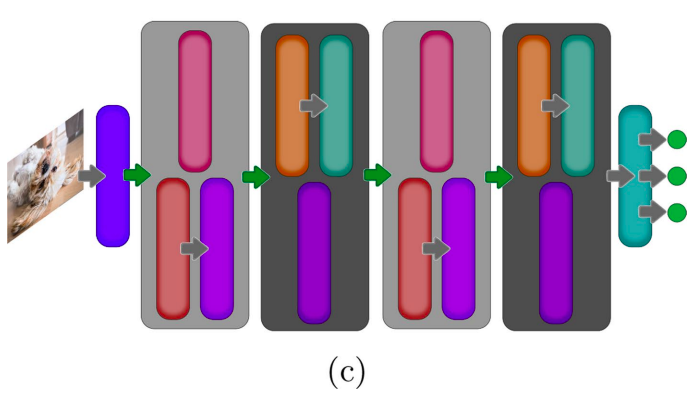
\includegraphics[width=0.5\textwidth]{images/ssp_cell_based.png}
        \caption{Exemplo de arquitetura Cell-based.}
    \end{figure}
    
\end{itemize}

\subsubsection{Como gerenciar o tamanho do SSp de forma eficiente?}

Com base na revisão sistemática, podemos separar as discussões e temas de SSp entre os seguintes tópicos:

\begin{itemize}
    \item \textbf{Adaptação dinâmica do SSp:} A abordagem mais simples é limitar manualmente a quantidade de camadas/conexões, porém os métodos mais modernos modificam o SSp durante a otimização, sendo guiados por hardware (uso de memória, latência e poder de processamento). O algoritmo FP-NAS é um exemplo, onde usa aprendizado probabilístico para analisar o SSp e reduzi-lo dinamicamente, resultando em um modelo que gasta menos memória e menos FLOPs.

    \item \textbf{Uso de variáveis contínuas:} Métodos que transformam o SSp discreto em um espaço contínuo; como exemplo temos o DARTS e CP-NAS. Cada possível conexão entre camadas tem uma variável contínua associada, então usa-se métodos baseados em gradiente, alterando os valores das conexões, dando pesos maiores para as conexões mais importantes.
    
    \item \textbf{Problema das restrições rígidas vs. Poda:} Ao restringir muito as opções, o algoritmo é forçado a procurar modelos com complexidades e profundidades específicas. A solução é que, em vez de começar com um SSp limitado, pode ser mais eficiente gerar células iniciais complexas e ao longo da busca aplicar técnicas de \textit{pruning} (podar as opções ruins dinamicamente).
    
    \item \textbf{Vantagem de limitar o SSp:} Se o objetivo final é colocar a rede em produção e integrar fluxos de MLOps em hardwares restritivos, a limitação prévia é vantajosa. Evita processamentos eternos (arquiteturas demasiadamente complexas sendo treinadas em hardwares não poderosos).
\end{itemize}

\subsection{\textit{Search Strategy} (SSt)}
A Estratégia de Busca (SSt) determina como explorar o SSp para encontrar o melhor modelo para um determinado \textit{dataset}. Ao longo dos anos, diversos otimizadores foram desenvolvidos; entre eles, alguns se destacam e são os mais utilizados (a "liderança" varia, assim como vemos na Figura 4).

\begin{figure}[h]
    \centering
    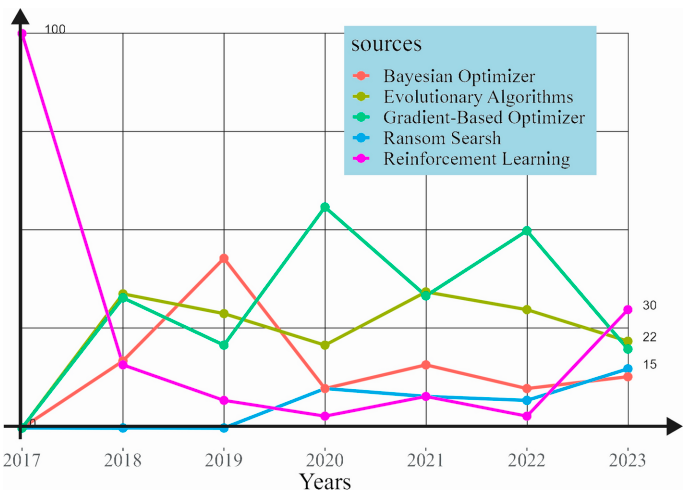
\includegraphics[width=0.8\textwidth]{images/top_optimizers.png}
    \caption{Evolução dos otimizadores mais utilizados ao longo dos anos.}
\end{figure}

O otimizador bayesiano ficou popular pela rápida convergência, mas a reformulação do SSp o tornou mais complexo. Os algoritmos evolucionários são alguns dos métodos mais populares e asseguram alta efetividade. Os baseados em gradiente ganharam mais popularidade com sua metodologia amigável a GPUs. O de busca aleatória é simples, mas não eficiente. O de aprendizado por reforço perdeu popularidade pelo alto custo computacional e longo tempo de validação, porém com o surgimento de rápidas e baratas técnicas de validação, reganhou destaque (a Figura 5 mostra uma tabela comparativa entre os otimizadores).

\begin{figure}[h]
    \centering
    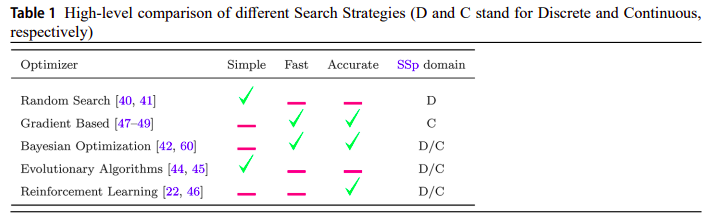
\includegraphics[width=0.8\textwidth]{images/optimizers_table.png}
    \caption{Comparação entre as estratégias de busca.}
\end{figure}

A descrição de cada otimizador é a seguinte:

\begin{itemize}[noitemsep]
    \item \textbf{\textit{Reinforcement Learning} (RL):} O algoritmo é treinado com uma recompensa/punição baseada no desempenho obtido na validação. No trabalho de Zoph e Le (\url{https://arxiv.org/abs/1611.01578}), o problema foi definido como um agente RL que busca otimizar um objetivo específico, como acurácia, por meio de seleção de componentes de arquitetura. Devido à necessidade de muitas validações, o método demanda muito poder computacional. 
    
    \item \textbf{\textit{Evolutionary Algorithms} (EA):} É uma classe de otimizadores baseados em princípios biológicos de evolução e genética. Algoritmo:
    
        \begin{itemize}
            \item População inicial: são algumas arquiteturas escolhidas.
            \item Avaliação de performance: pode ser feita por acurácia, complexidade e requisitos de hardware.
            \item Evolução da população: é feita por meio de técnicas de seleção para gerar a próxima geração.
            \item Critério de finalização: é predefinido como um número máximo de gerações ou um erro mínimo alcançado.
        \end{itemize}
    
    \item \textbf{\textit{Bayesian Optimization} (BO):} Utiliza modelos probabilísticos para aproximar a função objetivo e selecionar o próximo conjunto de hiperparâmetros. É eficiente quando a função objetivo não é contínua e/ou a avaliação é computacionalmente cara (minimiza o número de avaliações $\rightarrow$ \url{https://arxiv.org/abs/1806.10282}).
    
    \item \textbf{\textit{Gradient-based optimizer} (GO):} Depende da derivada ou do gradiente da função objetivo para atualizar os (hiper)parâmetros iterativamente. São considerados computacionalmente caros devido ao caráter iterativo, porém as GPUs aceleraram este processo (\url{https://arxiv.org/abs/1910.04465}).
    
    \item \textbf{\textit{Random Search} (RS):} É um método utilizado em problemas discretos (\url{https://arxiv.org/abs/1902.07638} e \url{https://arxiv.org/abs/1912.00848}). É simples, porém é o mais devagar dos otimizadores, logo tem uma aplicação limitada. É principalmente utilizado para estratégia de validação.
\end{itemize}

\subsection{Estratégia de Validação (Validation Strategy - VSt)}

É a etapa que mais consome tempo nos algoritmos NAS. Este ponto é o que retorna a performance de um modelo por meio de uma função objetivo e dá o retorno ao SSt e SSp. 

Existem vários métodos propostos na literatura, a abordagem mais direta é treinar cada modelo desde o início no dataset de treino e então avaliar a performance do modelo no conjunto de validação; ela é a mais correta, porém é muito custosa. Essa etapa às vezes é chamada de proxies, pois ela pode ser uma aproximação da performance do modelo no dataset, assim reduzindo o custo desta etapa (aproximar acelera o processo, ao invés de validar por completo).

Os métodos propostos podem ser classificados nas seguintes categorias:

\begin{itemize}[noitemsep]
    \item \textbf{\textit{Full Training}:} Cada arquitetura proposta pelo SSt é treinada por completo antes de avaliar a performance no conjunto de validação. Logo, ele compara as performances exatas dos modelos, mas com um custo de um treino longo e exaustivo.
    
    \item \textbf{\textit{Partial Training}:} Os modelos serão treinados por $r < n$ iterações. As $r$ iterações podem ser feitas para cada modelo desde o início (tipo 1) ou o modelo pode inferir os pesos a partir de outro modelo e então ser treinado por mais $r$ iterações extras (tipo 2). Ele reduz o processo de procura. Por exemplo, a performance de cada modelo pode ser avaliada após algumas épocas (\url{https://arxiv.org/abs/2006.13799}). O tipo 2, \textit{weight sharing} ou \textit{inheritance}, visa reduzir o tempo de treinamento compartilhando os pesos entre modelos; este processo possui quatro formas de implementação:
    \begin{itemize}
        \item Treinar uma vez uma arquitetura gigante e depois utilizar seus subsets como modelos menores (\url{https://arxiv.org/abs/1806.09055}).
        \item Treinar arquiteturas pequenas e então compartilhar seus pesos com uma arquitetura maior que tenha todos os pequenos modelos (\url{https://arxiv.org/abs/2104.00597}).
        \item Compartilhar pesos somente no momento de geração de um modelo por meio de modelos salvos (\url{https://arxiv.org/abs/2004.05565}).
        \item Transferir pesos de um modelo para outros modelos que são mais coerentes com algoritmos como o otimizador evolucionário (EA), em que o otimizador utiliza modelos prévios para gerar novos. Um exemplo famoso é o ENAS (\url{https://arxiv.org/abs/1802.03268}).
    \end{itemize}
    
    \item \textbf{\textit{Adaptive Training}:} O modelo treina completamente (\textit{from scratch}), mas o número de iterações depende do comportamento da curva de aprendizado. Esta mostra a acurácia ou a loss do modelo ao longo das iterações de treino. Exemplo que introduziu métricas de performance baseadas na profundidade e planidade (flatness) da loss durante o treinamento (\url{https://dynn-icml2022.github.io/papers/paper_11.pdf}).
    
    \item \textbf{\textit{No training (zero-shot)}:} Devido ao grande número de modelos treinados em um algoritmo NAS, o treino de cada um pode levar a um tempo de busca inviável. Então, métodos que produzam uma pontuação para cada modelo como um indicador de performance são desejados (tempo de validação tende a zero). Esse método é baseado em algoritmos relacionados aos dados do problema e/ou arquitetura do modelo (\url{https://arxiv.org/abs/2006.04647}).
\end{itemize}

A Figura 6 mostra uma tabela comparativa entre os métodos de validação.

\begin{figure}[h]
    \centering
    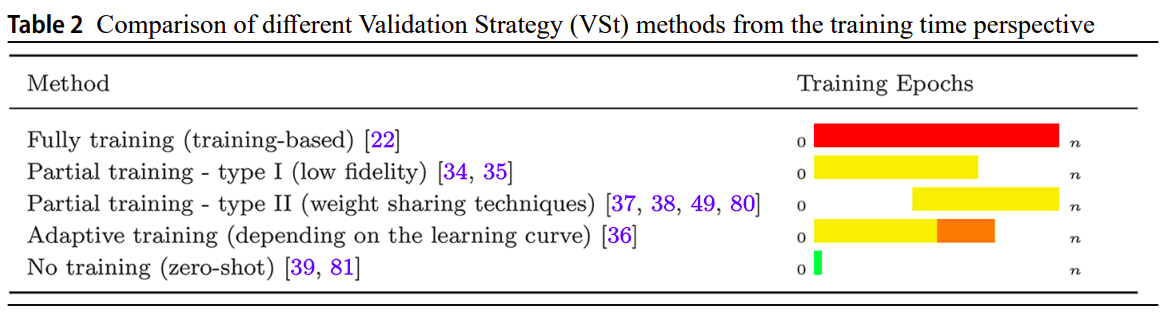
\includegraphics[width=0.8\textwidth]{images/vst_table_compare.png}
    \caption{Comparação entre os métodos de validação.}
\end{figure}

\end{document}